% npj Quantum Information-style companion manuscript.
% Structure follows Li et al., npj Quantum Inf. (2026), doi:10.1038/s41534-026-01365-1:
% Abstract -> Results -> Discussion -> Methods -> Data/Code availability -> References.
\documentclass[10pt]{article}

\usepackage[utf8]{inputenc}
\usepackage[T1]{fontenc}
\usepackage{amsmath,amssymb}
\usepackage{graphicx}
\graphicspath{{../QNet_Sim/results/experiments/figures/}}
\usepackage{hyperref}
\usepackage{booktabs}
\usepackage[margin=1in]{geometry}
\usepackage{cite}
\usepackage{caption}
\usepackage{setspace}
\usepackage{titlesec}

\captionsetup{font=small,labelfont=bf,labelsep=period}
\titleformat{\section}{\Large\bfseries}{}{0pt}{}
\titleformat{\subsection}{\normalsize\bfseries}{}{0pt}{}
\setstretch{1.08}
\newcommand{\muEL}{\mu_{\mathrm{EL}}}
\newcommand{\muEve}{\mu_{\mathrm{Eve}}}
\DeclareMathOperator{\hbin}{h_2}

\title{\textbf{Device-level parasitic emission as a routing constraint in
quantum networks: a VOA electroluminescence case study}}
\author{QiOpt4QNet Team\\
{\small\url{https://github.com/Sguy1908/QiOpt4QNet-Simulator}}}
\date{}

\begin{document}
\maketitle

\begin{abstract}
\noindent Entanglement-routing optimizers assume that a link is fully described by
a fidelity, a generation probability and a capacity. Hardware side channels
break that abstraction: Li \emph{et al.}\ recently showed that the forward-biased
$p$--$i$--$n$ variable optical attenuators (VOAs) in chip-based QKD transmitters
emit spontaneous electroluminescence near 1107~nm, which acts as a passive
Trojan-horse channel and as an independent noise source at the receiver.
Here we implement their analytic model, check it against the numbers they
publish, and couple it to a quantum-network simulator so that the same
allocators used for routing can be evaluated under the device effect. The
model reproduces the published mean photon numbers ($0.0048$, $0.0388$,
$0.0977$), an ideal reach of $\approx$320~km and a $\approx$50\,\% short-range
key-rate loss in the worst-case operating point. At network level the effect is
dominated not by fidelity loss (mean $\Delta F\le 0.011$ per link, $\le 6.1\,\%$
utility) but by security: with a 2.0~V, 1.6~ns drive, a security-blind exact
allocator admits requests of which $6.0$ of $7.45$ traverse links whose
passive-THA key rate is zero, and a security-aware allocator keeps only $2.0$ of
$7.75$ requests. A $10$~dB band-pass filter on the emission removes the
penalty. We also find that greedy allocators reorder their picks under
$10^{-6}$-scale fidelity perturbations. The device model is a reconstruction of
the published analysis, not a new measurement.
\end{abstract}

\section{Introduction}
Quantum networks distribute entanglement across repeater chains and grids, and
the routing layer decides which path and purification schedule each request
receives under memory and link-capacity limits. The optimizers studied in this
repository---an exact CP-SAT reference, greedy heuristics, a Metropolis
annealer, tensor-network compression and learned rankers---all consume a
per-link summary: raw fidelity, success probability, latency and capacity.

Implementation security is largely absent from that summary. Chip-based QKD is
usually analysed at the protocol level with idealised devices, yet integrated
photonic components combine classical and quantum functions in a tight
footprint. Li \emph{et al.}~\cite{li2026voa} identified one such mechanism: a
carrier-injection VOA is a lateral $p$--$i$--$n$ diode, so the recombination
that produces attenuation also produces light. They measured the emission
(centre wavelength inferred at $\approx$1078--1093~nm from an on-chip
interferometer, close to the 1107~nm silicon band gap), and analysed two
consequences: a \emph{passive Trojan-horse attack} (THA) when the VOA sits
upstream of the encoder, and a \emph{dual-source flaw} when it sits
downstream.

We ask a network-level question the original point-to-point study does not: when
links are driven by such transmitters, how much does the device effect change
what a routing optimizer should admit, and does it matter whether the optimizer
knows about it? Our contributions are (i) a tested implementation of the
published gain, QBER and THA-leakage expressions; (ii) a coupling of that model
to link fidelity and to a link-level security predicate; and (iii) a
controlled comparison of allocators on clean, security-blind and
security-aware instances, including the paper's proposed spectral-filter
mitigation.

\section{Results}
\subsection*{The device model reproduces the published numbers}
The model takes the VOA drive voltage $U$ and the signal pulse width $\Delta t$,
maps the measured emission count rate $C(U)$ to a mean photon number per pulse,
$\mu=-\ln[1-C(U)\Delta t]$ (Eqs.~\ref{eq:mu}), and propagates it through the
gain/QBER and leakage expressions in Methods. Using the two published count
rates (Table~\ref{tab:params}) it returns
$\mu_{\mathrm{Eve}}=0.0048,\ 0.0388,\ 0.0977$ for the paper's three operating
points, matching the reported values. Without parasitic light the decoy-state
BB84 rate is $0.099$ bit/pulse at zero distance and vanishes at
322~km, consistent with the $\approx$320~km reach in Fig.~6 of
ref.~\cite{li2026voa}. At $U=2.0$~V, $\Delta t=1.6$~ns the dual-source rate at
zero distance falls to $0.049$ bit/pulse (a $50\,\%$ reduction) and is
non-monotonic in distance, rising to $0.057$ at 5~km before falling, as in their
Fig.~8. The penalty relative to the ideal rate falls below $5\,\%$ by 20~km and below
$1\,\%$ by 30~km (at that level the comparison is limited by the difference
between the noise-aware and decoy-estimated single-photon bounds).

Two caveats. Only two count rates are published, so $C(U)$ is interpolated
log-linearly between $1.4$ and $2.0$~V (and extrapolated above), ramped linearly from
zero at the $0.8$~V turn-on to the $1.4$~V anchor, and set to zero below the turn-on;
intermediate voltages are model output, not data. And for the conventional GLLP
analysis the maximum passive-THA distances we obtain ($75.5$, $30.5$ and
$12.0$~km) are of the same order as, but not identical to, those read from
their Fig.~6; we did not have their numerical values or code, so we make no
claim of exact agreement there.

\begin{table}[h]
\centering
\caption{\textbf{Simulation parameters} (from Table~1 of
ref.~\cite{li2026voa} unless marked).}
\label{tab:params}
\small
\begin{tabular}{llll}
\toprule
Parameter & Symbol & Value & Note\\
\midrule
Misalignment error & $e_d$ & $0.0061$ &\\
Background yield & $Y_0$ & $2\times10^{-8}$ &\\
Detection efficiency (signal) & $\eta_{\mathrm{Bob}}$ & $0.78$ &\\
Error-correction inefficiency & $f_{\mathrm{EC}}$ & $1.2$ &\\
Fibre loss, 1550~nm / 1077~nm & $\alpha,\ \alpha'$ & $0.2$ / $0.8$~dB\,km$^{-1}$ &\\
Detection efficiency (EL) & $\eta'_{\mathrm{Bob}}$ & $0.25$ &\\
Signal / decoy intensities & $s,\ \nu,\ \omega$ & $0.48,\ 0.02,\ 0.001$ &\\
$C(1.4\,\mathrm{V})$, $C(2.0\,\mathrm{V})$ & & $2.38\times10^{7}$, $5.82\times10^{7}$~cps &\\
Sifting factor & $q$ & $1/2$ & $p_Z\to1$; ours\\
Link length range & $L$ & $2$--$30$~km & network study; ours\\
\bottomrule
\end{tabular}
\end{table}

\begin{figure}[h]
\centering
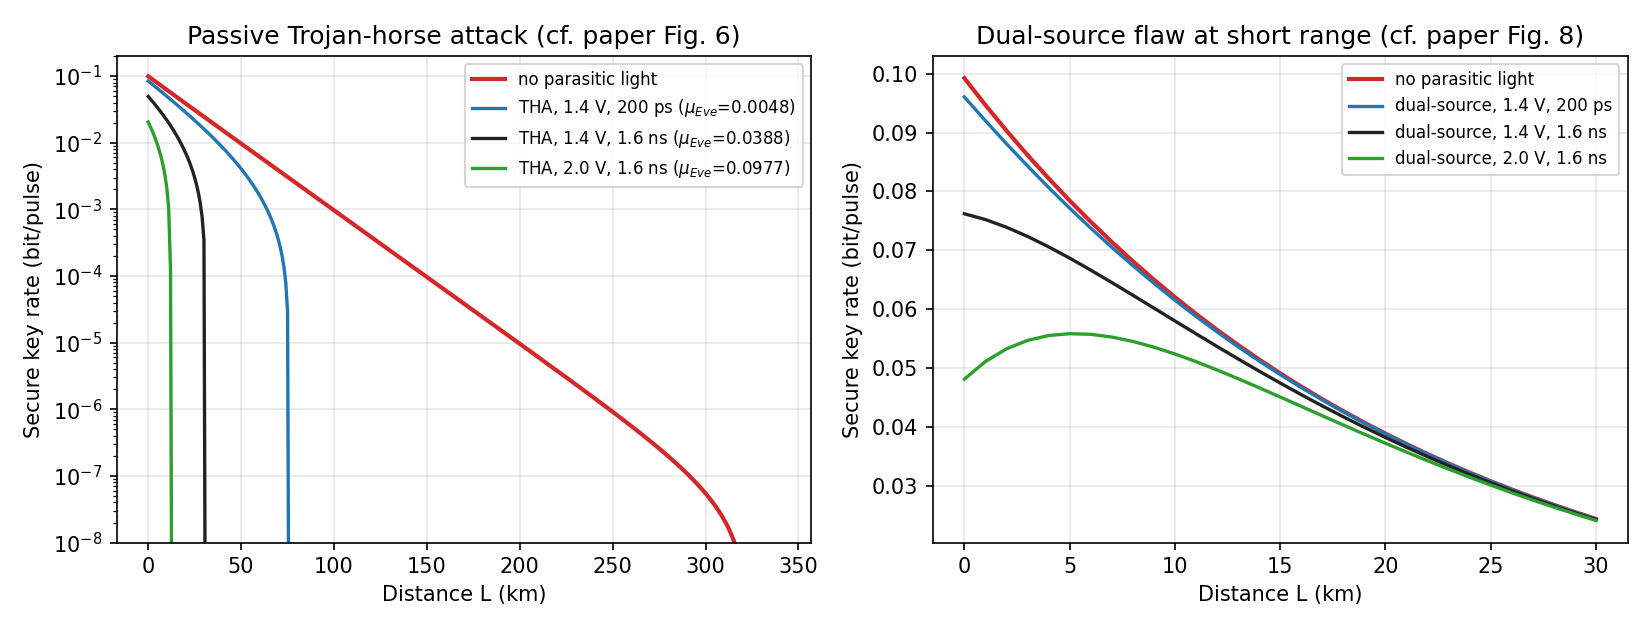
\includegraphics[width=\textwidth]{parasitic_key_rate.png}
\caption{\textbf{Secure key rate versus distance.} Left: passive THA for the
three VOA operating points, against the ideal decoy-state BB84 rate (red). Right:
dual-source flaw over the first 30~km, using the noise-aware single-photon
bound. $\muEve$ values are in the legend. The curves are our reconstruction of
the analysis in ref.~\cite{li2026voa}.}
\label{fig:keyrate}
\end{figure}

\subsection*{A noise-blind decoy estimator is not exploited in this reconstruction}
Ref.~\cite{li2026voa} argues that unmodelled parasitic clicks bias decoy-state
parameter estimation. We implemented that scenario by feeding the observed
(noise-inflated) gains to the standard two-decoy estimator (``naive'') and
compared it with a bound that uses the exact single-photon yield and error rate
in the presence of noise (``aware''). With Table~\ref{tab:params} the naive
estimate is \emph{lower} than the aware one everywhere ($\le 1.6\,\%$ at 0~km,
$0.9\,\%$ at 5~km), i.e.\ conservative. The key-rate loss in
Fig.~\ref{fig:keyrate} therefore comes from the added QBER and not from an
overestimate. This does not contradict the paper---which reports no explicit
expression for this case---but it means that the security-relevant part of the
dual-source flaw in our reconstruction is small, and we do not carry it into
the network study.

\subsection*{At network level the dominant effect is security, not fidelity}
We coupled the device model to the routing pipeline
(Methods). Each instance is a $3\times3$ grid or an 8-node chain with link
lengths drawn from $2$--$30$~km, raw link fidelity $0.92$, and $10$ requests; we
ran $10$ seeds per topology and each of the three VOA operating points, with the
exact CP-SAT allocator as reference and three greedy heuristics as robustness
checks. Each instance is solved three ways: \emph{clean} (no emission),
\emph{blind} (degraded links, the optimizer is unaware of the leak) and
\emph{aware} (bundles crossing a link with zero passive-THA key rate are
removed before allocation).

The fidelity channel is weak. The mean per-link loss is
$\Delta F=0.0005,\ 0.0042,\ 0.0105$ for the three operating points, and the
exact solver's utility falls by $0.1\,\%$, $1.7\,\%$ and $6.1\,\%$ relative to
clean (Table~\ref{tab:network}). It is larger only on short links: an
individual 2~km link at 2.0~V, 1.6~ns loses $\approx$0.04 in fidelity, while
a 25~km link loses $<0.002$.

The security channel is not weak. In the worst-case configuration $6.15$ of the
grid/chain links on average exceed the passive-THA reach ($12.0$~km), and the
blind exact allocator's solution routes $6.0$ of its $7.45$ admitted requests
over at least one such link---requests that it would report as successes while
their key is exposed. A security-aware allocator avoids those links and, because
they make up a large share of these sparse topologies, can serve only $2.0$ of
$7.75$ requests, a $74\,\%$ loss of admitted requests and $73.5\,\%$ of utility.
Neither of the two milder operating points produces an insecure link at these
lengths.

\begin{figure}[h]
\centering
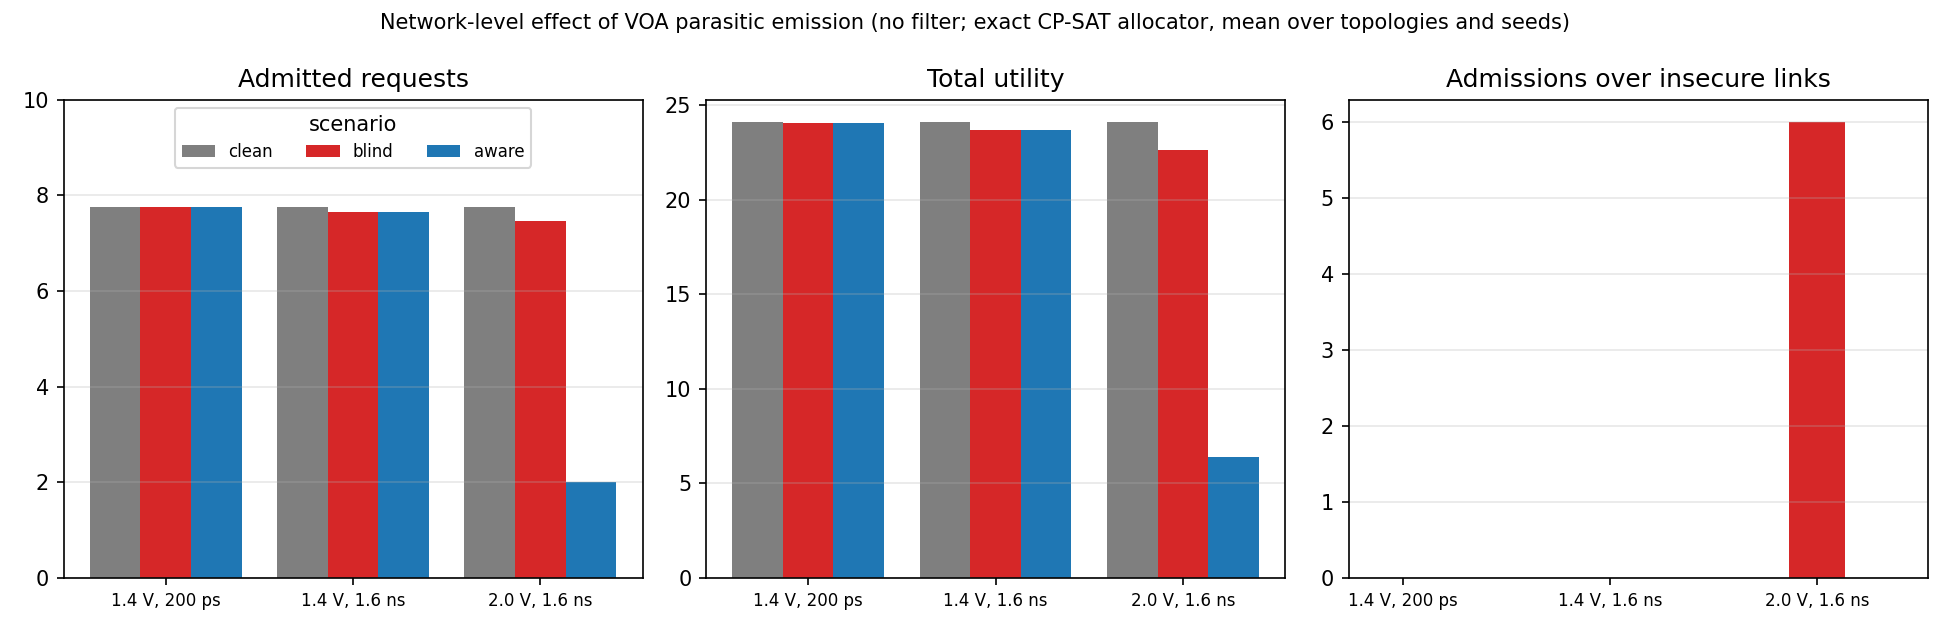
\includegraphics[width=\textwidth]{parasitic_network.png}
\caption{\textbf{Network-level effect of VOA parasitic emission.} Admitted
requests (left), total utility (middle) and admissions traversing an insecure
link (right) for clean, security-blind and security-aware allocation at the
three operating points, without a filter. Exact CP-SAT allocator, mean over both
topologies and 10 seeds. The ``clean'' bar is omitted from the right panel
because no light is emitted in that scenario.}
\label{fig:network}
\end{figure}

\begin{table}[h]
\centering
\caption{\textbf{Exact-allocator results without a filter} (mean over 2
topologies $\times$ 10 seeds; $n=20$ per cell).}
\label{tab:network}
\small
\begin{tabular}{lccccc}
\toprule
Operating point & $\Delta F$ & clean util. & blind util. & aware util. & blind insecure adm.\\
\midrule
1.4~V, 200~ps & 0.0005 & 24.11 & 24.09 & 24.09 & 0.0\\
1.4~V, 1.6~ns & 0.0042 & 24.11 & 23.71 & 23.71 & 0.0\\
2.0~V, 1.6~ns & 0.0105 & 24.11 & 22.63 & 6.40 & 6.0\\
\bottomrule
\end{tabular}
\end{table}

\subsection*{A band-pass filter removes the penalty}
Following the mitigation proposed in ref.~\cite{li2026voa}, we model a filter
after the VOA as a constant attenuation of the emission, scaling $\muEL$ and
$\muEve$ by $10^{-A/10}$. At the worst-case drive, $A=10$~dB brings the exact
solver back to $24.06$ of $24.11$ utility with no insecure link, and $A=20$~dB
to $24.10$ (Fig.~\ref{fig:filter}). We modelled the filter as a scalar and did
not model its insertion loss, bandwidth or the residual out-of-band
transmission of a real component.

\begin{figure}[h]
\centering
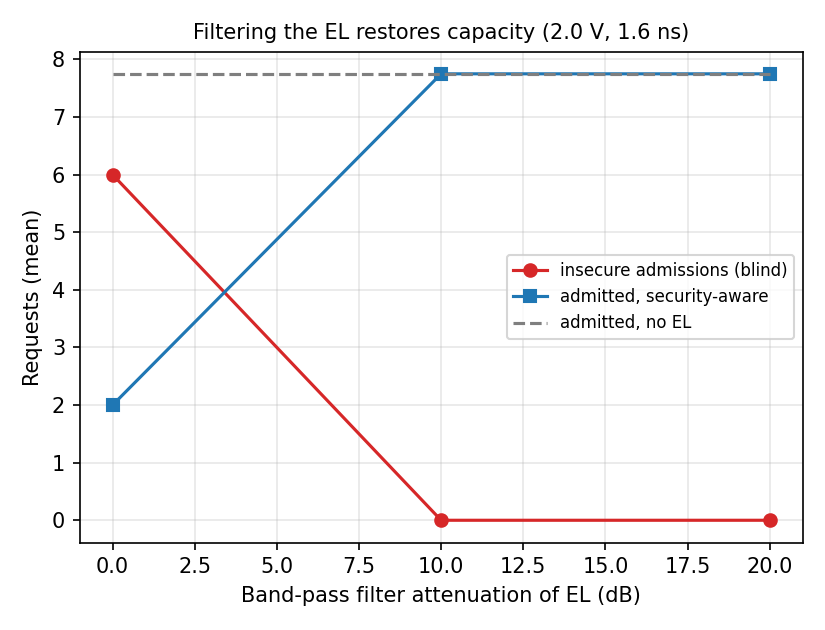
\includegraphics[width=0.55\textwidth]{parasitic_filter.png}
\caption{\textbf{Effect of filtering the emission} at 2.0~V, 1.6~ns. Insecure
admissions of the blind allocator (red) and requests admitted by the
security-aware allocator (blue) versus filter attenuation, against the no-EL
level (grey). Only three attenuation values were simulated.}
\label{fig:filter}
\end{figure}

\subsection*{Greedy allocators are brittle to negligible fidelity changes}
With a $20$~dB filter the mean per-link fidelity change is
$\Delta F\lesssim10^{-4}$ (as small as $3\times10^{-6}$ in individual
instances), yet the greedy heuristics
still admit $0.1$--$0.2$ fewer requests on average than in the clean scenario,
whereas the exact allocator loses none ($7.75$ vs $7.75$). The bundle lists
are identical or nearly identical in size; a perturbation of the utility of order $10^{-6}$ reorders
ties and the greedy pick cascade diverges. This is a property of the
heuristics, not of the physics, and is why we report the exact allocator as the
reference and the per-allocator breakdown separately
(\texttt{parasitic\_network\_by\_allocator.csv}).

\subsection*{Summary of the routing framework}
For context, the surrounding framework (detailed in the companion
paper~\cite{qiopt4qnet}) formulates bundle selection as a QUBO and benchmarks
a Metropolis annealer, tensor-network compression and OpenJij against an exact
ILP. Reported there: mean $1.5\,\%$ optimality gap for the Metropolis annealer;
a request-conditioned penalty calibration that tightens capacity coefficients on
$12.9\,\%$ of $1{,}080$ instances; chance-constrained fidelity requirements that
expose a $5$--$14\,\%$ implicit violation rate in the deterministic rule;
local-repair recourse with up to $1065\times$ speedup over replanning; and
conflict-aware purification scheduling matching per-request throughput on
$85\,\%$ of instances at $2.06\times$ lower Bell-pair cost. The present study
adds a device-level layer beneath those results.

\section{Discussion}
We turned a point-to-point hardware finding into a routing question and found
that the useful answer is a security predicate on links, not a fidelity
correction. For the two operating points nearest to typical use the effect on
the optimizer is small: the fidelity term is at most a few percent and no link
is insecure at metropolitan lengths. The worst-case drive matters because
the passive-THA reach ($12$~km) falls inside a plausible metropolitan link
distribution; the model then implies that a routing layer that ignores the leak
reports secure service that is not secure.

Several limitations bound these statements.
(i) All device inputs are taken from a single published study; we did not
measure any device, and our reconstruction of the two-decoy estimator and the
$C(U)$ interpolation are our own. (ii) The map from QBER to Werner fidelity
($F=1-\tfrac32\,\mathrm{QBER}$) and the choice to treat every link as a
BB84-style detector link are modelling assumptions of this repository, not of
the paper; entanglement-swapping links with memories would differ. (iii) The
``insecure link'' predicate uses the worst-case ideal Eve of the paper (unit
efficiency, no dark counts), so it is conservative. (iv) The network instances
are small ($9$ and $8$ nodes, $10$ requests), the length distribution is
uniform, and $n=20$ per cell, so the absolute utility numbers should not be
extrapolated; the qualitative split between a small fidelity effect and a large
security effect is what we consider robust. (v) The filter is a scalar
attenuation.

The main practical recommendation is architectural: carry a per-link security
attribute---here a boolean derived from the key rate---through bundle generation,
and treat it as a hard constraint in the optimizer, rather than as a fidelity
correction after the fact. Extending the same interface to other parasitic
emitters (phase modulators, on-chip detectors) is a natural next step, as
suggested in ref.~\cite{li2026voa}.

\section{Methods}
\subsection*{Emission and leakage model}
The mean photon number per signal window is
\begin{equation}
\mu=-\ln\!\bigl[1-C(U)\,\Delta t\bigr],\label{eq:mu}
\end{equation}
with $C(U)$ the VOA emission count rate (Table~\ref{tab:params}); for
the passive THA $\muEve=\mu$ under an ideal, dark-count-free unit-efficiency
detector. For a coherent copy of the four BB84 polarisations the basis
dependence is
\begin{equation}
\Delta=\tfrac12\Bigl[1-e^{-\muEve}\bigl(\cosh\tfrac{\muEve}{\sqrt2}
+\tfrac12\sinh\tfrac{\muEve}{\sqrt2}\bigr)\Bigr],\label{eq:delta}
\end{equation}
and the phase-error bound of the GLLP--Koashi analysis is
\begin{equation}
e_X'=e_X+4\Delta'(1-\Delta')(1-2e_X)+4(1-2\Delta')\sqrt{\Delta'(1-\Delta')e_X(1-e_X)},
\qquad \Delta'=\Delta/Y_1,
\end{equation}
set to $1/2$ if $\Delta'\ge\tfrac12$. The passive-THA key rate is
\begin{equation}
R=q\Bigl\{Q_1\bigl[1-\hbin(e_X')\bigr]-Q_s f_{\mathrm{EC}}\,\hbin(E_s)\Bigr\},
\end{equation}
with $Q_1=s\,e^{-s}Y_1^{L}$, $Y_1^{L}$ and $e_X=e_1^{U}$ from the two-decoy
estimator~\cite{ma2005practical} applied to the clean gains, and $q=1/2$.

\subsection*{Dual-source gain and QBER}
For signal intensity $\gamma$, transmittances $\eta$ (signal) and $\eta'$
(parasitic), $s_c=1-e^{-\gamma\eta}$ and $n_c=1-e^{-\muEL\eta'}$:
\begin{align}
Q&=1-(1-Y_0)(1-s_c)(1-n_c),\\
EQ&=Y_0e_0+e_ds_c+e_0n_c-Y_0e_0e_ds_c-Y_0e_0^2n_c-e_de_0s_cn_c
+Y_0e_0^2e_ds_cn_c,
\end{align}
with $e_0=1/2$ (the paper's Eqs.~23--24). The exact single-photon yield and
error rate used in the ``aware'' bound follow by setting the signal photon number
to one in the same construction.

\subsection*{Network coupling}
For a link of length $L$, raw fidelity $F_0$ and $e_d=\tfrac23(1-F_0)$, let
$E(\muEL)$ be the QBER above at intensity $\gamma=s$. The degraded fidelity is
\begin{equation}
F=\max\bigl\{0.25,\ F_0-\tfrac32\,[E(\muEL)-E(0)]\bigr\},
\end{equation}
so a link without emission is unchanged exactly. A link is \emph{insecure} if
the passive-THA key rate at $L$ is $0$. A bundle is removed in the
security-aware scenario if any of its edges is insecure. A filter of $A$~dB
multiplies $\mu$ by $10^{-A/10}$.

\subsection*{Instances and statistics}
Topologies: $3\times3$ grid and 8-node chain, edge capacity $4$, memory $8$,
raw fidelity $0.92$. Per-link lengths are drawn uniformly from $2$--$30$~km
(seeded, identical across scenarios). Requests: $10$ per instance, minimum
fidelity uniform in $[0.5,0.9]$, weights uniform in $[0.5,5]$, three candidate
paths per request, purification levels $0$--$2$. Allocators:
\texttt{cp\_sat\_exact} (reference), \texttt{utility\_per\_resource\_greedy},
\texttt{congestion\_aware\_greedy}, \texttt{greedy\_local\_search}. Seeds
$0$--$9$. Values are means over 20 instances per cell. Paired differences
(clean minus blind exact-solver utility) are non-zero in all $20$ instances at
every operating point, with mean $\pm$ standard error $0.02\pm0.002$,
$0.40\pm0.10$ and $1.48\pm0.35$ utility units for the three operating points; we
did not run formal significance tests.

\section*{Data availability}
All CSVs and figures are under \url{QNet_Sim/results/experiments/}:
\url{parasitic_key_rate.csv}, \url{parasitic_summary.csv},
\url{parasitic_network.csv}, \url{parasitic_network_summary.csv} and
\url{parasitic_network_by_allocator.csv}.

\section*{Code availability}
Model: \url{QNet_Sim/src/hardware/parasitic_emission.py} and
\url{QNet_Sim/src/hardware/parasitic_network.py}. Experiment:
\url{QNet_Sim/experiments/run_parasitic_emission.py}. Tests (24):
\url{QNet_Sim/tests/test_parasitic_emission.py} and
\url{QNet_Sim/tests/test_parasitic_network.py}.

\section*{Author contributions, competing interests, funding}
\emph{To be completed by the authors.}

\begin{thebibliography}{9}
\bibitem{li2026voa} Li, Z.\ \emph{et al.} Security risks of VOA-induced
luminescence in chip-based quantum key distribution. \emph{npj Quantum Inf.}
(2026), doi:10.1038/s41534-026-01365-1.
\bibitem{ma2005practical} Ma, X., Qi, B., Zhao, Y.\ \& Lo, H.-K. Practical decoy
state for quantum key distribution. \emph{Phys.\ Rev.\ A} \textbf{72}, 012326
(2005).
\bibitem{qiopt4qnet} QiOpt4QNet Team. Quantum-inspired optimization for
entanglement routing in quantum networks: from QUBO solver families to
chance-constrained stochastic scheduling. Companion manuscript,
\texttt{paper/qiopt4qnet\_paper.tex}, this repository.
\end{thebibliography}

\end{document}
